\section{Representación de Rotaciones Espaciales}
La aplicación más importante de los cuaterniones en la computación gráfica y la robótica es la representación de rotaciones tridimensionales. A diferencia de las matrices de rotación o los ángulos de Euler, los cuaterniones unitarios (aquellos cuya norma es $\lVert q \rVert = 1$) evitan el problema del \textit{Gimbal Lock} (bloqueo del cardán), son más eficientes computacionalmente y permiten realizar interpolaciones esféricas (SLERP) de forma suave al calcular trayectorias.

\subsection{Ángulos de Euler: Roll, Pitch y Yaw}
Antes de introducir la fórmula con cuaterniones, es fundamental comprender la notación estándar de orientación utilizando ángulos de Euler, comúnmente llamada convención Roll-Pitch-Yaw. Esta convención describe la orientación de un cuerpo rígido en el espacio mediante tres rotaciones sucesivas alrededor de los ejes de un sistema de coordenadas de referencia:

\begin{itemize}
    \item \textbf{Roll (Alabeo - $\phi$):} Es la rotación alrededor del eje $X$. En un vehículo, describe la inclinación lateral (de lado a lado).
    \item \textbf{Pitch (Cabeceo - $\theta$):} Es la rotación alrededor del eje $Y$. Describe la inclinación hacia adelante o hacia atrás.
    \item \textbf{Yaw (Guiñada - $\psi$):} Es la rotación alrededor del eje $Z$. En el cálculo de la odometría de una base móvil, este es el ángulo más importante, ya que define hacia dónde está apuntando (girando) en el plano horizontal.
\end{itemize}

\subsection{Rotación de un Vector con Cuaterniones}
Para rotar un vector tridimensional $\mathbf{v} \in \mathbb{R}^3$ un ángulo $\theta$ alrededor de un eje de rotación arbitrario definido por un vector unitario $\mathbf{u} = (u_x, u_y, u_z)$, utilizamos un cuaternión unitario $q$. 

El cuaternión $q$ que codifica esta rotación se construye de la siguiente manera utilizando la notación escalar-vectorial:
\begin{equation}
    q = \left( \cos\left(\frac{\theta}{2}\right), \, \mathbf{u} \sin\left(\frac{\theta}{2}\right) \right)
\end{equation}

En su forma polinomial, esto equivale a:
\begin{equation}
    q = \cos\left(\frac{\theta}{2}\right) + \left( u_x \sin\left(\frac{\theta}{2}\right) \right)i + \left( u_y \sin\left(\frac{\theta}{2}\right) \right)j + \left( u_z \sin\left(\frac{\theta}{2}\right) \right)k
\end{equation}

Para aplicar la rotación al vector $\mathbf{v}$, primero debemos convertir dicho vector en un cuaternión puramente imaginario (es decir, con parte escalar igual a cero): $v_q = 0 + v_xi + v_yj + v_zk$. 

Luego, el vector rotado $\mathbf{v}'$ se obtiene mediante el \textbf{producto de emparedado} (sandwich product) utilizando el cuaternión $q$ y su conjugado $q^*$:
\begin{equation}
    v_q' = q v_q q^*
\end{equation}

El resultado $v_q'$ será otro cuaternión puramente imaginario, cuyas componentes vectoriales corresponderán al vector $\mathbf{v}'$ rotado.

\textbf{Ejemplo:}

Imaginemos que estamos analizando la cinemática de un robot y queremos rotar un vector de posición inicial $\mathbf{v} = (1, 0, 0)$ (apuntando a lo largo del eje $X$) aplicando un giro de $90^\circ$ ($\frac{\pi}{2}$ radianes) puramente en Yaw (alrededor del eje $Z$). 

1. Definimos el eje de rotación y el ángulo:
   $\mathbf{u} = (0, 0, 1)$ y $\theta = \frac{\pi}{2}$.

2. Construimos el cuaternión unitario $q$:
   Dado que $\cos(\frac{\pi}{4}) = \frac{\sqrt{2}}{2}$ y $\sin(\frac{\pi}{4}) = \frac{\sqrt{2}}{2}$, obtenemos:
   \begin{equation*}
       q = \frac{\sqrt{2}}{2} + \left(0 \cdot \frac{\sqrt{2}}{2}\right)i + \left(0 \cdot \frac{\sqrt{2}}{2}\right)j + \left(1 \cdot \frac{\sqrt{2}}{2}\right)k = \frac{\sqrt{2}}{2} + \frac{\sqrt{2}}{2}k
   \end{equation*}

3. Calculamos el conjugado $q^*$:
   \begin{equation*}
       q^* = \frac{\sqrt{2}}{2} - \frac{\sqrt{2}}{2}k
   \end{equation*}

4. Convertimos el vector a rotar en un cuaternión puro $v_q$:
   \begin{equation*}
       v_q = 0 + 1i + 0j + 0k = i
   \end{equation*}

5. Aplicamos la fórmula de rotación $v_q' = q v_q q^*$. Primero calculamos $q v_q$:
   \begin{align*}
       q v_q &= \left( \frac{\sqrt{2}}{2} + \frac{\sqrt{2}}{2}k \right) (i) \\
       &= \frac{\sqrt{2}}{2}i + \frac{\sqrt{2}}{2}ki \\
       &= \frac{\sqrt{2}}{2}i + \frac{\sqrt{2}}{2}j \quad (\text{ya que } ki = j)
   \end{align*}

6. Multiplicamos el resultado por $q^*$:
   \begin{align*}
       v_q' &= \left( \frac{\sqrt{2}}{2}i + \frac{\sqrt{2}}{2}j \right) \left( \frac{\sqrt{2}}{2} - \frac{\sqrt{2}}{2}k \right) \\
       &= \frac{2}{4}i - \frac{2}{4}ik + \frac{2}{4}j - \frac{2}{4}jk \\
       &= \frac{1}{2}i - \frac{1}{2}(-j) + \frac{1}{2}j - \frac{1}{2}(i) \quad (\text{sustituyendo } ik = -j, \: jk = i) \\
       &= \frac{1}{2}i + \frac{1}{2}j + \frac{1}{2}j - \frac{1}{2}i \\
       &= j
   \end{align*}

El cuaternión resultante es $0 + 0i + 1j + 0k$, lo cual corresponde al vector rotado $\mathbf{v}' = (0, 1, 0)$. Como era de esperarse físicamente, rotar el vector unitario del eje $X$ un ángulo de $90^\circ$ alrededor del eje $Z$ hace que termine alineado exactamente sobre el eje $Y$.


\subsection{Diagrama del Proceso de Rotación}
Para consolidar los conceptos anteriores, el siguiente diagrama de bloques ilustra el flujo de cálculo computacional necesario para aplicar una rotación a un vector en el espacio utilizando cuaterniones. Esta estructura modular demuestra cómo los datos de entrada se transforman antes de operar el producto de emparedado.

\vspace{0.5cm}

\begin{figure}[hbt!]
    \centering
    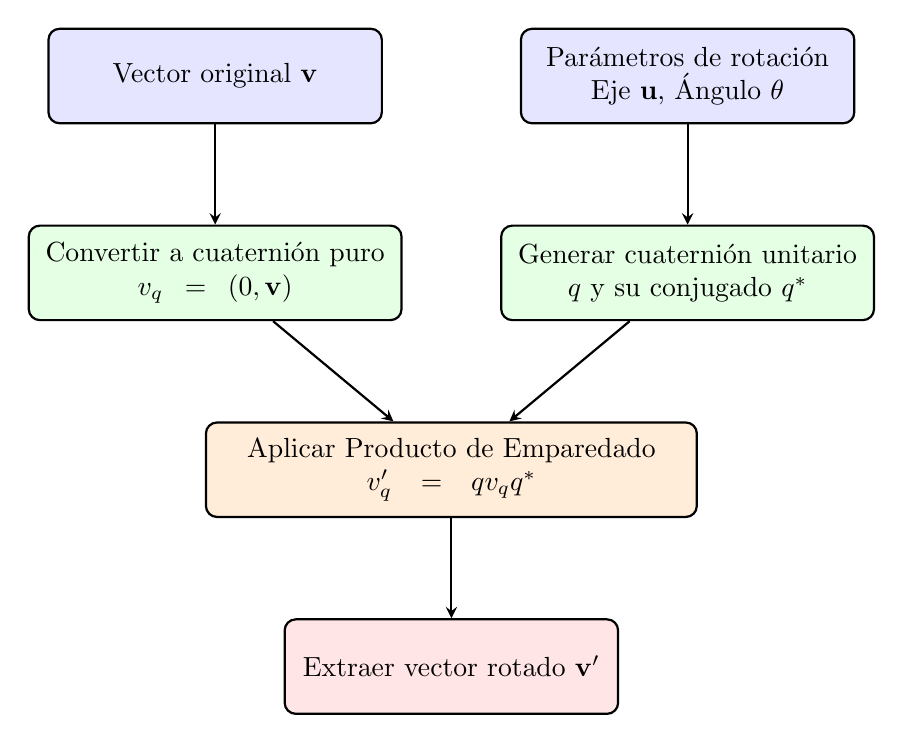
\begin{tikzpicture}[>=stealth, thick,
        box/.style={rectangle, draw, rounded corners, text centered, minimum height=1.2cm}]

        % Nodos de Entrada
        \node[box, fill=blue!10, text width=4cm] (vec_in) at (0, 0) {Vector original $\mathbf{v}$};
        \node[box, fill=blue!10, text width=4cm] (rot_in) at (6, 0) {Parámetros de rotación \\ Eje $\mathbf{u}$, Ángulo $\theta$};

        % Nodos de Conversión
        \node[box, fill=green!10, text width=4.5cm] (vec_quat) at (0, -2.5) {Convertir a cuaternión puro \\ $v_q = (0, \mathbf{v})$};
        \node[box, fill=green!10, text width=4.5cm] (rot_quat) at (6, -2.5) {Generar cuaternión unitario \\ $q$ y su conjugado $q^*$};

        % Nodo de Operación Central
        \node[box, fill=orange!15, text width=6cm] (sandwich) at (3, -5) {Aplicar Producto de Emparedado \\ $v_q' = q v_q q^*$};

        % Nodo de Salida
        \node[box, fill=red!10, text width=4cm] (vec_out) at (3, -7.5) {Extraer vector rotado $\mathbf{v}'$};

        % Conexiones con flechas direccionales
        \draw[->] (vec_in) -- (vec_quat);
        \draw[->] (rot_in) -- (rot_quat);
        \draw[->] (vec_quat) -- (sandwich);
        \draw[->] (rot_quat) -- (sandwich);
        \draw[->] (sandwich) -- (vec_out);

    \end{tikzpicture}
    \caption{Diagrama de bloques del flujo para rotar un vector utilizando cuaterniones.}
    \label{fig:diagrama_rotacion_cuaterniones}
\end{figure}




\subsection{Conversión entre Cuaterniones y Ángulos de Euler}
Aunque los cuaterniones son computacionalmente superiores para operar rotaciones, los ángulos de Euler (Roll, Pitch, Yaw) son mucho más intuitivos para el análisis humano y son el formato estándar que entregan muchos sensores inerciales. Por ello, es indispensable saber convertir entre ambas representaciones.

Supongamos que tenemos un cuaternión unitario definido como $q = q_0 + q_1i + q_2j + q_3k$ (donde $q_0$ es la parte escalar) y los ángulos de Euler definidos como Roll ($\phi$), Pitch ($\theta$) y Yaw ($\psi$).

\subsubsection{De Ángulos de Euler a Cuaternión}
Para construir un cuaternión a partir de tres rotaciones sucesivas, se calcula el cuaternión individual de cada eje y se multiplican en el orden específico de la convención utilizada (generalmente Yaw, luego Pitch, luego Roll). El cuaternión resultante se calcula con las siguientes ecuaciones:

\begin{align}
    q_0 &= \cos\left(\frac{\phi}{2}\right)\cos\left(\frac{\theta}{2}\right)\cos\left(\frac{\psi}{2}\right) + \sin\left(\frac{\phi}{2}\right)\sin\left(\frac{\theta}{2}\right)\sin\left(\frac{\psi}{2}\right) \\
    q_1 &= \sin\left(\frac{\phi}{2}\right)\cos\left(\frac{\theta}{2}\right)\cos\left(\frac{\psi}{2}\right) - \cos\left(\frac{\phi}{2}\right)\sin\left(\frac{\theta}{2}\right)\sin\left(\frac{\psi}{2}\right) \\
    q_2 &= \cos\left(\frac{\phi}{2}\right)\sin\left(\frac{\theta}{2}\right)\cos\left(\frac{\psi}{2}\right) + \sin\left(\frac{\phi}{2}\right)\cos\left(\frac{\theta}{2}\right)\sin\left(\frac{\psi}{2}\right) \\
    q_3 &= \cos\left(\frac{\phi}{2}\right)\cos\left(\frac{\theta}{2}\right)\sin\left(\frac{\psi}{2}\right) - \sin\left(\frac{\phi}{2}\right)\sin\left(\frac{\theta}{2}\right)\cos\left(\frac{\psi}{2}\right) 
\end{align}

\subsubsection{De Cuaternión a Ángulos de Euler}
Para extraer la orientación intuitiva a partir de un cuaternión, aplicamos trigonometría inversa sobre combinaciones específicas de sus componentes. En programación y robótica, es crucial utilizar la función $\text{atan2}(y, x)$ en lugar de $\arctan$ regular para preservar el cuadrante correcto de los ángulos:

\begin{align}
    \text{Roll } (\phi) &= \text{atan2}\big(2(q_0 q_1 + q_2 q_3), 1 - 2(q_1^2 + q_2^2)\big) \\
    \text{Pitch } (\theta) &= \arcsin\big(2(q_0 q_2 - q_3 q_1)\big) \\
    \text{Yaw } (\psi) &= \text{atan2}\big(2(q_0 q_3 + q_1 q_2), 1 - 2(q_2^2 + q_3^2)\big)
\end{align}

\textit{Nota sobre singularidades:} Cuando el ángulo Pitch ($\theta$) se acerca a $\pm 90^\circ$ ($\pm \frac{\pi}{2}$), el término dentro del arcoseno tiende a $\pm 1$, lo que desencadena la singularidad conocida como \textit{Gimbal Lock}. En las implementaciones prácticas de software, se suele incluir una condición para manejar este caso límite, forzando los valores de Roll y Yaw de manera manual para evitar inestabilidades numéricas.

